\section{Discussion}
A Wizard of Oz study has been conducted following the A-B1-C-B2 case study design with a single participant.  In Phase A, the parent alone prompted the child through hand-washing steps.  In Phase B1, the robot alone prompted the child.  In Phase C, the parent and the robot jointly prompted.  In Phase B2, the robot alone prompted the child again.  Parent researcher interview was conducted during breaks between trials.  Both qualitative and quantitative analyses were conducted on the study data, and we observed promising results.

\subsection{List of Thesis Contributions}
\begin{itemize}
	\item Demonstrated the feasibility of robot based prompting system for children with ASD in guiding them through hand-washing
	\item Exhibited one viable way of robot prompting to children with ASD in the task of hand-washing using verbal and gestural prompts as modes of interactions, which was similar to the parent prompts
	\item Discovered the importance of a training phase consisting of the parent robot joint prompting in increasing child's compliance to robot prompts
	\item Identified the challenges and their possible solutions to building and testing an ABA framework based robot prompting system for children with ASD
	\item Created and validated an efficient video coding scheme for analyzing children with ASD's behavior in response to hand-washing prompts
\end{itemize}	


\subsection{Summary of Results}
We saw that, although the child did not listen to the robot as much as he did to the parent when the robot was first introduced, through a parent robot joint training phase, the child showed drastic improvement in robot prompt compliance, approaching the compliance level achieved by the parent prompts.  Although our participant did not appear to need help in how to execute each hand-washing steps, he did need prompting to get the hand-washing started and stay on task, and supervision on scrubbing, rinsing and drying longer and not getting too much soap.  Our analyses showed that through training, the robot was successful in getting the child to meet most of these goals.  Specifically, the qualitative analyses showed that the child waited for the robot to prompt first before starting the hand-washing activity.  Also, the child followed the robot's rinse prompts and rinsed longer as a result.  However, the robot was only somewhat successful in getting the child to move on from the soap step, and was unsuccessful in getting the child to scrub hands or to dry hands longer.  The parent, on the other hand, had no problems in getting the child to scrub hands, but she did have some difficulties in getting the child to dry longer and had definite difficulties in getting the child to move on from the soap step.

%\subsection{Quantitative Analysis and Results - Further}
%After qualitative analysis, we saw that the child improved in robot prompts compliance through the training Phase C and retained those improvements in Phase B2.  Specifically, the greatest improvements were that the child was waiting for the turn on water robot prompt before executing, the child complied more to robot rinse prompts, and not terminating by himself as much during rinsing.  
%
To further validate these qualitative findings further and quantify the improvements, we here created and analyzed the following measures:
\begin{itemize}
	\item \textbf{Not Waiting For Turn On Water Prompt Rate}: the percentage of trials in a phase that the child does not wait for the turn on water prompt from the robot (i.e. starts executing that step by himself).
	\item \textbf{Rinse Step Complied Prompt Rate}: the percentage of prompts for the rinse steps in a trial that the child followed by showing an effort of attempt.
	\item \textbf{Longest Duration of Rinse Step}: the longest duration in seconds in a trial that the child rinses hands continuously without terminating.
\end{itemize}
\subsubsection{Not Waiting For Turn On Water Prompt Rate}
The Not Waiting For Turn On Water Prompt Rate for Phase A is 6 out of 16 trials = 37.5\%, for Phase B1 is 5 out of 8 trials = 62.5\%, for Phase C is 5 out of 21 trials = 23.8\%, for Phase B2 is 2 out of 5 trials = 40\%.  We see an improvement of the child in waiting for the robot's turn on water prompt in training Phase C, and a retained improvement (although with a slight slide back) in Phase B2.

\subsubsection{Rinse Step Complied Prompt Rate}
The Rinse Step Complied Prompt Rate is plotted in Figure \ref{fig:5CompliedPromptRate-RinseStep}, and has a median for Phase A of 100\%, for Phase B1 of 33\%, for Phase C of 100\%, for Phase B2 of 75\%.  Despite variance in data, we see that the improvement in rinse step robot prompt compliance is retained in Phase B2.
\begin{figure} [H]
	\centering
	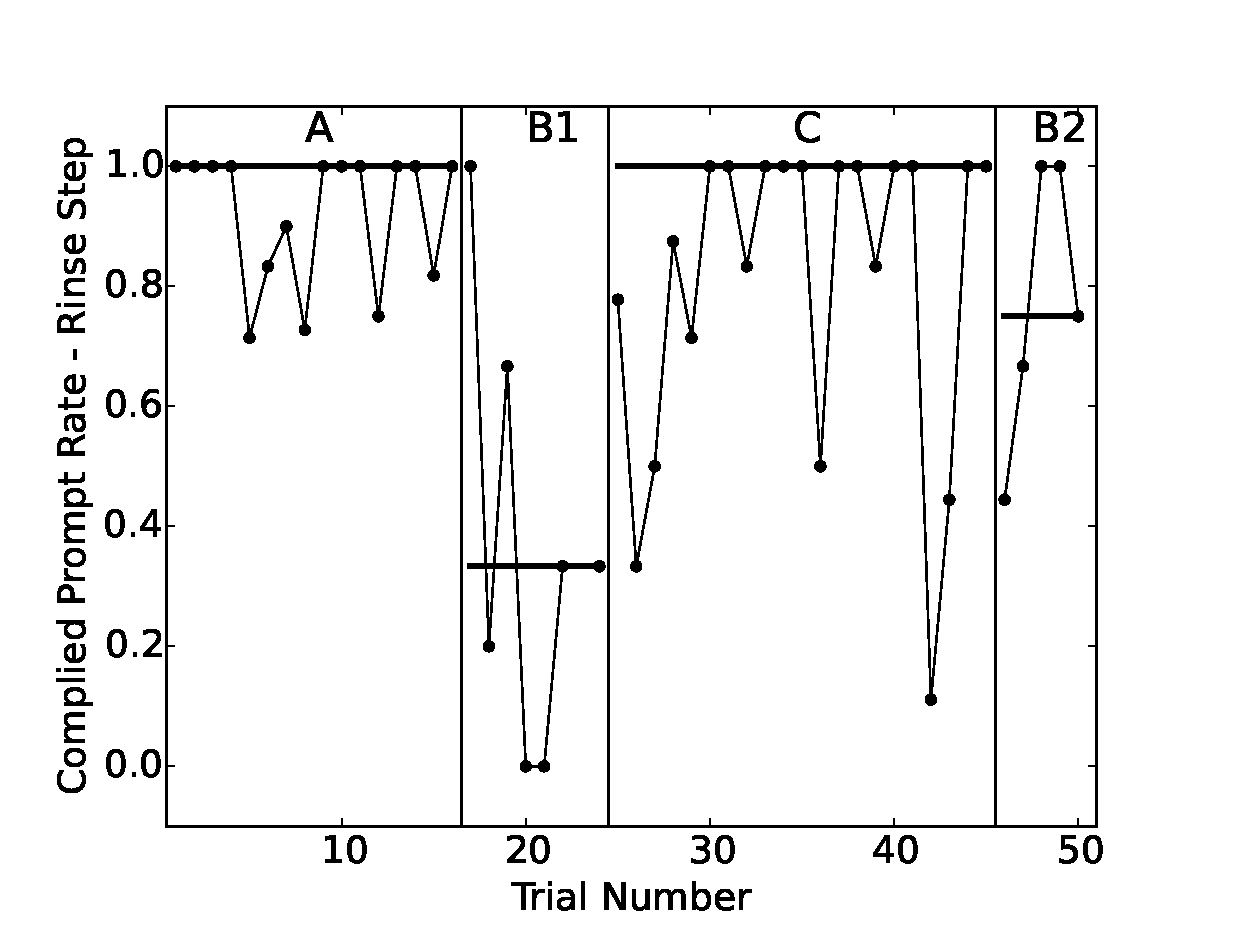
\includegraphics[width=0.6\textwidth]{./img/data_analysis/5CompliedPromptRate-RinseStep.eps}
	\caption{Rinse Step Complied Prompt Rate}
	\label{fig:5CompliedPromptRate-RinseStep}
\end{figure}

\subsubsection{Longest Duration of Rinse Step}
The Longest Duration of Rinse Step is plotted in Figure \ref{fig:8LongestDurationofRinsesec}, and has a median for Phase A of 7.15s, for Phase B1 of 2.87s, for Phase C of 5.36s, and for Phase B2 of 7.09s.  We see that the rinse step duration in Phase B1 was especially short, and was improved in Phase B2.
\begin{figure} [H]
	\centering
	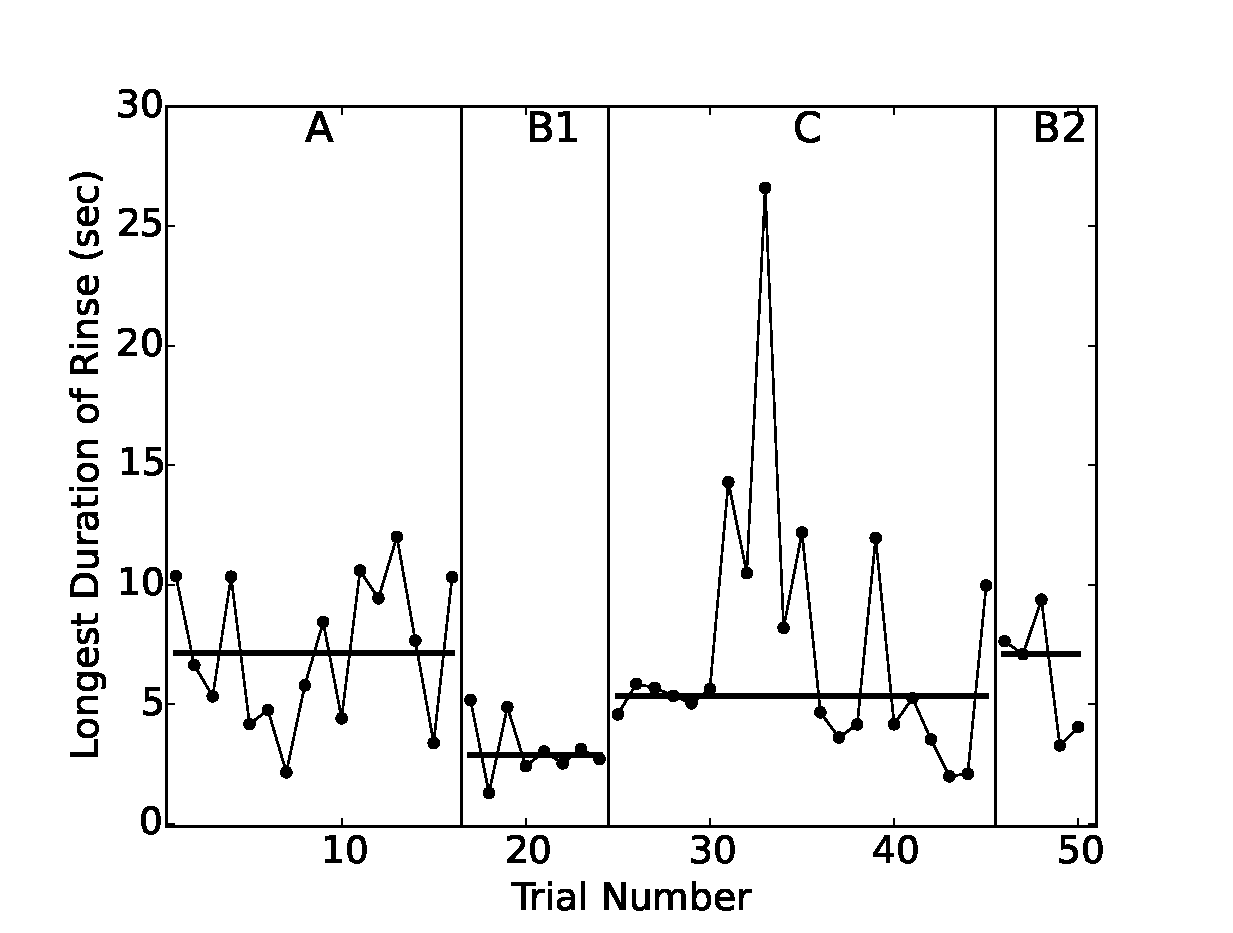
\includegraphics[width=0.6\textwidth]{./img/data_analysis/8LongestDurationofRinsesec.eps}
	\caption{Longest Duration of Rinse Step}
	\label{fig:8LongestDurationofRinsesec}
\end{figure}
In whole, these confirm the finding that the child's improvements in responding to robot in training Phase C are retained in Phase B2.

The way the robot prompted was verified to be very similar to how the parent prompted.  The parent was not instructed in the specifics of how to prompt -- she prompted in the most natural way she and the child were used to, and yet there were a lot of similarities between the parent and the robot's prompting patterns.  First, they shared similar breakdown of the hand-washing steps, although the parent referred to the scrub step as lather.  In addition, both the parent and the robot prompted by giving verbal instructions along with some form of gesture prompts.  The differences were that the parent used more pointing and less motion demonstration, and that the motion demonstrations from the parent were much faster moving than the robot's (especially for the scrub step).  The child paid much more attention to the parent's faster moving motion demonstrations than the robot's, and is one area of future improvements.  Other design recommendations for the robot included faster response times to child's behaviors, issuing a fast attention grabber accompanied with increased severity in tone of voice when the child is non-compliant, and rewarding the child for major steps only (e.g. the end of rinsing and drying steps).  Other design recommendations raised by the parent and the researcher mainly involved engaging the child better, including more dynamic motions for gestures, playing cartoon noises for rewards or attention grabbers, having a bigger robot so it is more visually engaging, etc.

In terms of modes of interactions needed between the child and the robot for successfully helping the child to wash hands, the delivering of verbal and gestural prompts with at least two levels of severity (more severe sounding and looking prompts delivered when the child is non-compliant) were definitely needed.  However, the detection of the visual focus of attention of the child showed little value.  The child's visual attention was hardly an indicator of engagement at all.  On the other hand, we found that understanding verbal feedbacks from the child may be useful as the child verbally repeated instructions when he was processing them, and murmured back in protest when he did not wish to follow certain prompts.  Utilizing these speeches as indication of the child's engagement may be useful in adjusting robot prompts to better suit the child's needs.  Also, we observed that the child did not like prolonged rinsing, and what the parent did was to stop prompting the rinse step and to move on to the next step when the child showed non-compliant behavior through rinsing for only a second and quickly removing his hands from the water.  The robot did not move on and repeated the rinse prompts in hope the child would follow, and as a result, the child often moved on by himself without waiting for the robot.  In future studies, the robot should also implement a way to work with the child to rinse as much as possible but learn to move on when the child shows signs of non-compliance.


\subsection{Internal and External Validity}
In this section, our results are critically reviewed based on data collection, analysis methods, and result interpretations.  Possible sources of errors, competing interpretations, limitations of results, and their generalizability are discussed.

\subsubsection{Quantitative Analysis Method}
The choice of measures used in the quantitative analyses were based on our study objectives and chosen in light of the qualitative analysis results, in an attempt to answer the question ``Is the robot NAO able to guide our participant, a child with ASD, through hand-washing?".  ``Number of Steps Completed'' only reflected the variety of steps completed, but did not measure the quality of the completed steps.  Thus it could only partially confirm how well the robot guided the child.  ``Longest Duration of Rinse Step'' was our attempt to measure the quality of the rinse step completed.  The rinse step was chosen due to the drastic improvement the child exhibited on this particular step, and the duration of the longest rinse was the most obvious way to measure the quality of the rinse step completion.  One thing to note is, the parent, during the training phase, focused most of her prompts on getting the child to follow the rinse prompts from the robot, but very little prompts were focused on the dry hands prompts.  Consequently, we did not experience as much improvement on the duration of dry hands step.  To link the child's success in completing all steps and with good quality to the prompting agents, the ``Complied Prompt Rate'' and the ``Ignored Prompt Rate'' were measured, for all steps (and Complied Prompt Rate for the rinse step particularly as well).  We see that the robot had much more influence on the child in Phase B2, but not in Phase B1, and this resulted in an increased duration of rinse in Phase B2.  Thus, we concluded that the robot was successful in improving the quality of hand-washing of our child with ASD.  But since the child already knew all the steps and was able to complete all steps in Phase B1 with minimal influence from the robot, no conclusions can be made regarding whether the robot could successfully teach our child with ASD a new hand-washing step.

Medians were used as a fair and reliable way of comparing the measures across phases.  The choice of median, as opposed to mean, was out of the consideration for robustness against outliers.  This may be a good choice if the data had relatively low variance and few outliers.  However, our data contained high variance, and the definition of outliers became blurred.  Take ``Rinse Step Complied Prompt Rate'' (seen in Figure \ref{fig:5CompliedPromptRate-RinseStep}) for example.  The rate in Phase C has a median of 100\%, but there are a third of data points in this phase falling below 80\%.  Thus, one obvious question is, why have we not used some form of description of variance alongside our description of data centers (i.e. median) in our across phase comparisons?  The reasoning was that the low sample size for some phases (e.g. Phase B2 only has 5 data points) made any analysis based on variance not statistical significant.  This is a limitation of our study results, but given the pilot nature of our study, it is acceptable since it yielded promising results confirming the direction of future studies.

Another limitation exists in our lack of control on video data annotation errors.  For a more rigorous future study, more than one person should carry out the data annotations, and the degree of annotator subjectiveness can then be characterized by an inter-rater agreement measure such as the Cohen's Kappa \cite{volkmar2005handbook}.

\subsubsection{Qualitative Analysis Method}
The qualitative analyses of our study employed several strategies to ensure internal validity.  These strategies being reviewed include triangulation, member checks, adequate engagement in data collection, reseracher's position or reflexivity, peer review / examination, audit trial, rich thick description, an maximum variation \cite{merriam2014qualitative}.  Firstly, we employed triangulation by using multiple investigators and sources of data to confirm findings.  The observations of the child's behaviors and possible robot design recommendations were made by the researcher through making field notes of the trials video data, by the parents through the parent researcher interview discussions and the post intervention survey.  Secondly, during the parent researcher interviews, due to the interactive nature of the interview format, the member check technique was inherent.  The researcher was able to check his understanding of the emerging findings with the parent to ensure minimal misinterpretation was made.  In regards to researcher's position or reflexivity, the researcher was trained mainly in the engineering discipline and had limited experience and expertise in teaching children with ASD.  Such lack of experience may prove invalid any opinion the researcher had on the child's behaviors and on the reasons behind them.  However, the researcher relied heavily on the parents' interpretation of the child's behaviors, preferences, and possible reasons behind his behaviors instead.  The parents, being both experienced with the child's needs in particular and trained with knowledges of children with ASD in general, were very adequate observers used by our study.  In addition, audit trail and rich, thick descriptions were used to compensate the researcher's interpretation errors.  By providing a detailed account of the backgrounds, methods, procedures, and decisions made when conducting the study, the value of the study results can be critically assessed based on contexts by other researchers themselves when reading this thesis.  Lastly, during the training phase, the parent involvements were purposefully varied through the phase.  This maximum variation technique allowed greater diversity in sample selection, enabling a greater range of findings and possible applications of the findings.

In whole, the study was mostly carried out and analyzed rigorously.  However, the study was limited in that we did not collect data to saturation.  Phase A and Phase B1 were carried out long enough to see saturation of findings, but due to limitation of time, training Phase C and Phase B2 were not carried long enough to such saturation.  Especially, the training Phase C could have been longer to see possibly even further improvement of the child, and the second phase C could have been longer (at least to match the length of Phase B1) to eliminate any doubts that the improvements observed in training phase were successfully retained.

\subsubsection{Confounding Variables}
Due to the study protocol and the research design, there were several uncontrolled variables that may have confounded our results, threatening the internal validity of our results.

One confounding variable was the change of robot control scheme in the middle of Phase B1.  The reason for change was because our participant required a much more reactive robot who can switch the current step being prompted on the fly.  As stated in the study protocol, if any essential improvements of the robot (or the study procedures) were made apparent through the ongoing analysis, we would implement the change.  After the control scheme switch, both the parent and the robot operator (the researcher) felt the robot was more responsive to the child.  However, the parent did report that the robot was still too slow for the child, and sometimes the pause between robot actions were still too long.  This confounding variable had a sudden change, and we expected to also see sudden changes in our dependent measures shortly following the effect.  However, this was not observed, and may be due to the effect size of this confounding variable was too low compared to the level of noises in our measures.  Another possibility is that some inherent nature of the child made him remaining to behave a certain way despite changes in stimulus.  Either way, this confounding variable does not threaten our results that the robot was eventually able to help the child through hand-washings.  However, it may threaten the hypothesis that it was the training phase instead of the robot control scheme change that caused the improvements in the child's behaviors towards the robot.

Another confounding variable was the fact that the current study (Wizard of Oz) involved a human operator (the researcher) remotely controlling the robot.  The researcher had no experience guiding the participant through hand-washing prior to the study, and thus it was a learning process for the researcher through out the study as well.  This meant that the researcher changed the order of steps the robot prompts were delivered to best fit the child's preference (e.g. the child preferred to put on soap before turning on water).  Also, the researcher chose prompts that were more effective (e.g. the attention grabber was not effective and so was not used in the end, and the child did not distinguish between scrub hands and rinse hands, so scrub hand prompts were not used in the end).  These changes were gradual, but may play a confounding effect on our measures, threatening the hypothesis that the training phase was the sole cause of the child's improvements.  In addition, in the future when we will be automating the robot behaviors, tuning the robot prompts and order of steps to each child's preference will be an inevitable part of the automation process.

The researcher was not the only one learning, the child in fact was learning and familiarizing with the robot prompts, the experiment environment, and the hand-washing activity in this environment.  Children with ASD are very particular about keeping routines in a familiar environment.  Thus, introducing the robot, which the child did not have any prior experience to playing with or following orders from, in a foreign washroom with unfamiliar washroom setups, created a barrier for the child to put on his best responses to the robot prompts.  Since the parent alone prompting phase (Phase A) also had the unfamiliarity of environment confounding effect, this confounding variable does not threaten the conclusion that the robot did not perform as well as the parent as a prompting agent.  But the reason for this inequality in performance can be explained by the robot being inferior to the parent as a prompting agent by nature, or can be explained by the fact that the child was much used to following orders from the parent than the robot.  In addition, the child's unfamiliarity and learning to get used to being prompted by and following the robot, was also the alternative explanation of his improvements, competing with the training phase explanation.  Lastly, the child was already skilled in most of the hand-washing steps, thus little learning or improvements over the completion of steps were observed.  Instead, the only rooms for improvements were on the quality of step completion for scrubbing, rinsing, and drying.  Thus, our result that the robot was able to improve the child's rinse duration may have been confounded by the fact that the child could have improved in this regard with or without the robot's presence.  However, our results that the child did not recede to shorter rinse durations in Phase B2 (when being prompted alone by the robot) remained unchallenged by this confounding variable.

The last confounding variable is fatigue.  This variable was identified by the parents as well as the researcher when observing the child's behaviors.  Because of the number of repetitions of hand-washing conducted as well as the long durations of rinse in each hand-washing, the child quickly became fatigued and unwilling to comply to rinsing and sought to finish the remaining of the steps as quickly as possible.  This confounding variable introduced noises to our measures, burying important patterns that may have otherwise been observed.  In future studies, long duration of rinse (around 12 seconds) can still be required, but the repetitions must be avoided by having less than five hand-washings each day and spread them sparsely through the day.  Logistically, this would mean conducting the research in a school or home wash-room, where the child carries everyday activities, rather in a laboratory.

\subsubsection{Generalizability}
Our study only had one participant.  This means our results may only be applicable to this particular child, but not generalizable to the ASD population.  The next study in the future should increase the number of participants while validating the major results of the current study.  The single subject research design should be used for this future study, since due to the diverseness of the children with ASD population, measures may have different levels across subjects.  Thus, we should generalize the effectiveness of an intervention by comparing the amount of change of measure levels for each child when having the intervention compared against that same child not having the intervention.  Also, the secondary aim of this future study is to find out the participant demographics of a subpopulation of children with ASD that our intervention works consistently well on.  Only after this future study validating our major results and after we choose a subpopulation to focus on, should we attempt a larger scale randomized control trial, in which we divide the participants into control and intervention groups, and generalization of intervention effectiveness is made by directly comparing the measure levels between groups.  The focus of this randomized control would be to show clinical effectiveness of our intervention on the focused subpopulation.

The robot showed promising results in supervising our child with ASD, who already knew the basics of the hand-washing steps, but only needed guidance on the initiation and termination of steps.  It is still unknown how our robot would perform in teaching children with ASD the motions of hand-washing steps.  The parents and the researcher were not satisfied with the robot's dexterity, and worried that this lack of complexity of the robot's hands would not be adequate in teaching the child complex hand-washing motions such as scrubbing or drying.  Future study should explore this aspect further with children with ASD who have not learned the specifics of hand-washing step motions yet.

One more limitation existed in our experiment protocol, specifically in regulating how the parent prompts in Phase C.  During Phase C, where the parent prompts the child alongside the robot, we gave the parent freedoms to decide how best to prompt.  Firstly, the parent could choose between verbal prompting in competition with the robot prompts, verbal prompting complementary to robot prompts, and physical prompting complementary to robot prompts [sec ref].  The parent decided to focus on the latter two, and alternated between the two as she saw fit.  Secondly, the parent could decide when to prompt relative to robot prompts.  In general, the parent prompted immediately after the robot.  However, there are cases where the parent prompts simultaneously with the robot, or even before the robot.  Our result that Phase C acted as a training phase that resulted in effectiveness improvement of robot prompts still holds.  What it does affect, though, is that we do not know which variable regarding how the parent prompts in Phase C was most beneficial in improving robot prompt effectiveness.  Thus, in future experiments, controlling how the parent prompts in the training phase is needed to better understand how to consistently improve robot prompt effectiveness.

In addition, the intensity of our training, although very repetitive in each visit, was very sparse in a weekly schedule.  There was only one visit each week, and the training only lasted two weeks.  It was our hypothesis that, if we implemented a more intensive training, maybe three times a day, seven days a week, and maybe for a month of duration, we would achieve complete independence of parent in using the robot to guide the child through hand-washing.  Longitudinally focused intensive training may be one possible direction of future study.

Our study was conducted in the washroom of the HomeLab, in the Toronto Rehab Institute.  This experimental setting is a controlled environment, where camera can be installed anywhere we desired to best capture and analyze the study.  The use of camera is essential for the robot (or the operator) in tracking and understanding the child's progress during the hand-washing.  Eventually, when the robot is automated, the operator will be replaced by AI and computer vision algorithms, which will still rely on the cameras as sensor input.  The parents raised the concern that installing cameras on the washroom wall, in the way we did in our study, was not possible at the home settings.  They voiced that they are willing to make the compromise of having their child with ASD being under the camera in the washroom if this will help him independently execute ADLs, but they are not willing to have any other member of the family under the camera.  The solution to this would be to have a mobile robot that follows the child with ASD, and the camera will be attached onto the robot instead of fixed in the washroom.  The feasibility of such setup was not tested in our study, and should be employed in future studies, in the home or in the laboratory settings.

In whole, we learned from our study that the robot was a promising prompting agent in supervising the child with ASD through hand-washing.  It is not hard to hypothesize that such success can be replicated in other ADLs such as tooth-brushing, putting on clothes, or cooking.  Future studies may investigate the robot's effectiveness in prompting these other ADLs.  However, one immediate question follows: is robot the best prompting agent available for helping children with ASD through ADLs?  The successes we had with the robot prompts were mainly due to its ability to deliver verbal and gesture prompts.  However, a multimedia system with a LCD monitor could deliver similar prompts, by having a virtual avatar displayed on screen carrying out the robot prompts the same way.  The key difference lies that such system lacks embodiment in the physical world.  It may be worthwhile to compare the impact of this embodiment in effectiveness of the prompting agent in future studies.  If similar effectiveness is observed, the virtual avatar prompting agent may be the cost effectiveness solution that may be commercially available to families with children with ASD immediately.

%\subsection{Research Significance}
%significance:	
%	- what gaps have we achieved to fill in our study results?  should we continue this line of research? why or why not?  in what direction should we best continue?
%	- also discuss how are the results related to literature and what research gap it fills, i.e. significance of results (might need generalization analysis), talk about scientific contribution of our study and results
%	- The value this thesis is not only the conclusions it might make, but also the methodology.  Basically, it's the first study of its kind, and employed new analysis framework instead of adopting existing methodology.  Took me a while to do the video annotation framework.  Need to emphasize this contribution's significance.

\subsubsection{Challenges and Recommendations}
Because of the preliminary nature of our study, the results were not significant.  However, through conducting the study, we have learned some of the challenges we must face to succeed in studies of this sort and gained some insights on how to solve these challenges.  We here summarize the challenges met and their recommendations.

There are three aspects of things we would like to achieve:
\begin{enumerate}
	\item Increasing prompt compliance and engagement of COACH
	\item Designing the behaviors of a Socially Assistive Robot (SAR) for children with ASD
	\item Building an in-vivo Assistive Technology for Cognition (ATC) for children with ASD based on the Applied Behavior Analysis (ABA) / Discrete Trial Training (DTT) framework
\end{enumerate}

There are challenges faced in relation to each aspect.  Specifically, for (1), we do not know how to measure engagement for children with ASD.  In addition, we did not design the study for statistical significance when comparing participant compliance to robot prompts versus to caregiver prompts.  Lastly, we did not design the study to show if robot prompts are better than video prompts in engagement and compliance.

For (2), to build a SAR, design decisions need to be made in balancing the objectives of prompting the task and of engaging the user.  In the context of prompting children with ASD through hand-washing, our study showed a working way of robot prompting using verbals and gestures that were similar to the caregiver's.  The challenge lied in how to engage the child to look at the prompts, and how to engage the child in the activity of hand-washing in general.

For (3), the challenges setup wise include the child being unfamiliar with the experimental environment (i.e. the washroom) and with the robot, and the repetitiveness and a lack of natural motivation of the trials.  The challenges study design wise include the need for clinically significant sample size and a more specific inclusion criteria controlling participant's hand-washing level (based on the amount of assistance they need).  Also, the study design needs to control for learning effect when comparing between robot versus parent (versus video) prompts compliance.  In addition, the training phase needs to be formalized so that the caregiver can follow a reproducible protocol in prompt fading and reinforcement schedule.  Lastly, testing the maintenance of hand-washing skill acquisition without the ATC and across settings should be reported.

These challenges should be taken into consideration when designing future studies.  An extensive account of the challenges we faced, along with some recommendations made targeting these challenges, are presented in tabular form and reorganized into methodological challenges (Table \ref{tab:MethodChallenge}), population-specific challenges (Table \ref{tab:PopulationChallenge}), and technical challenges (Table \ref{tab:TechnicalChallenge}).
\begin{longtable}{ | p{5cm} | p{10cm} | }
	\hline
	\textbf{Challenge Encountered}	&	\textbf{Potential Solution / Recommendation} \\	\hline
	Child did not engage with robot when presented alone 	&	Have an introduction session prior to the start of the robot phases, where the caregiver introduces the robot as the helper for washing hands, and give some opportunity for the robot to interact with the children as a group briefly in an engaging activity, such as singing / dancing.  Also, conduct a training phase where the caregiver teaches each child to follow the robot prompts during hand-washing.	\\	\hline
	Training phase needs to be formalized so that the caregiver can follow a reproducible protocol in prompt fading and reinforcement schedule	&	The training phase's overall aim is to fade caregiver's involvement systematically until the child is able to wash hands needing only robot prompts.  The caregiver involvement can be broken into these levels, in decreasing order: caregiver behind child and guide child in following robot prompts, caregiver behind child and correct child behaviors through nudging (or guiding if nudging ineffective) in following robot prompts, caregiver stand beside child and correct child behavior physically in following robot prompts (nudging or guiding), caregiver stand beside child and correct child behavior through pointing (and physically if pointing ineffective) in following robot prompts.  Positive reinforcement should be given immediately after the completion of every get soap step, rinse step, and dry step.	\\	\hline
	Need to control the confounding effects of the child learning as the study progresses in our comparison of prompt compliance and task execution.  In addition, need to test for maintenance of skill acquisition in absence of ATC	&	We propose a five phase study that has two variations: A-B-C-D-A and A-C-D-B-A.  Phase A is the baseline phase, where the caregiver tests the child's hand-washing skill, lets the child to wash hands by themselves and only help if the child shows no progress in twenty seconds.  The caregiver offers no prompts, and only helps by completing the stuck step for the child.  Phase B is the parent prompt phase, where the parent proactively prompt each step.  Phase C is the robot parent training phase, where the robot proactively prompt while the parent instructs the child to follow the robot prompts.  Phase D is the robot prompt phase, where the robot proactively prompt each step.  The reason we repeat phase A again in the end is to test for skill acquisition in absence of ATC, and quantify the learning effect of the study as a whole.  The reason we have two variations of the phases, and each child randomly assigned to one of the variations, is to counter balance the learning's confounding effect on our comparison of prompt compliance and task execution between robot and parent.  The reason we do not have two robot prompt phases flanking the training phase (unlike the WoZ conducted in this thesis) is because the necessity of the training phase has already been shown by this thesis.  However, a study devoted to comparing different forms of the training phase on robot prompt compliance and task executions may also be beneficial.	\\	\hline
	Need to collect data to saturation for all phases and the sample size for each phase needs to be statistically significant, and the need to include statistical analysis in the study	&	Using c-statistics for analysis, the study with minimum of eight trials per phase or as many trials as needed for the child's behavior to be stabilized for each phase should be conducted.	\\	\hline
\caption{Methodological Challenges}
\label{tab:MethodChallenge}
\end{longtable}


\begin{table}[H]
	\centering
	\begin{tabular}{ | p{5cm} | p{10cm} | }
		\hline
		\textbf{Challenge Encountered}	&	\textbf{Potential Solution / Recommendation} \\	\hline
		Do not know how to measure engagement	&	This thesis attempted to investigate if the child is more engaged when prompted by a humanoid robot.  However, the literatures offered little clues on how to measure engagement level for children with ASD.  Possible features that reveal engagement should couple with sensory inputs that is salient to the individual, and may vary across individuals.  For our participant, visual attention was a poor indicator of engagement.  Instead, verbal feedback was seen as a possible indicator.  For future studies, survey / interview to caregiver may be used to gather clues of what is a good indicator of engagement for each individual participant.  Also, visual attention, verbal feedbacks, among other forms of interactions, may be candidates for engagement level indicator.	\\	\hline
		Child unfamiliarity with washroom and robot, fatigue to repetitiveness and lack of natural motivation of the trials, need for clinically significant population sample size	&	Conduct the study in an autism school, where trials are only conducted when natural motivations arise for hand-washing.  The trials should be conducted on a daily fashion, integrated into the child's daily routine, over a period of more than a month	\\	\hline
		More specific inclusion criteria controlling participants' hand-washing levels	&	The current inclusion criteria are appropriate except missing one criteria - participant hand-washing level.  Children with ASD have varying abilities of daily of living skills.  Specifically for hand-washing, the child may require prompts on how to execute each step, or on which steps to do next, or simply just on initiating the hand-washing activity and being reminded to be on task when distractions occur.  Future studies should select one group of users based on this classification, and design robot behaviors specifically for this group.	\\	\hline
	\end{tabular}
	\caption{Population-specific Challenges}
	\label{tab:PopulationChallenge}
\end{table}


\begin{table}[H]
	\centering
	\begin{tabular}{ | p{5cm} | p{10cm} | }
		\hline
		\textbf{Challenge Encountered}	&	\textbf{Potential Solution / Recommendation} \\	\hline
		Do not know how the robot can better engage the child to look at prompts and in the activity in general	&	The robot can be more visually engaging by exhibiting greater range of motion, faster, and more animated gestures.  Also, cartoon sounds and flashing LEDs can also be used to engage the child in general, for example, as rewards.	\\	\hline
		Child does not wait for prompts due to robot prompt delays	&	Minimize pause between robot gestures / verbal prompts, and create shorter versions of the prompts for the extended steps (e.g. rinse step) so the shorter prompts are repeated in a rapid manner (e.g. every two seconds).	\\	\hline
		Child does not comply to prompts	&	Need a more severe version of each prompt (shorter verbal prompt with more commanding posture for gesture, may include the child's name in the verbal prompt), which is used when child is not complying to prompts.  Also need a “call for caregiver prompt” so that the child learns that his/her noncompliance is the reason for caregiver's interventions.	\\	\hline
		Child sometimes gets too much soap	&	Need a “stop getting soap” prompt	\\	\hline
		Operator is unfamiliar with the child's behaviors and hand-washing habits, and the robot control needs to be tested out before the start of the study	&	Record the parent prompt phase (Phase B) and have the operator practice controlling the robot using the recorded videos so that the robot is able to prompt each step proactively just like the parent.	\\	\hline
	\end{tabular}
	\caption{Technical Challenges}
	\label{tab:TechnicalChallenge}
\end{table}
